\section{Auswertung}
\label{sec:Auswertung}

\begin{table}[!htp]
\centering
\caption{Die gemessenen Temperaturen zu den jeweiligen Zeitpunkten.}
\label{tab:zeit-temp}
\begin{tabular}{
  S[table-format=4.0] @{${}\pm{}$} S[table-format=1.0]
  S[table-format=3.1] @{${}\pm{}$} S[table-format=1.1]
  S[table-format=3.1] @{${}\pm{}$} S[table-format=1.1]}
\toprule
\multicolumn{2}{c}{$t$ / s} & \multicolumn{2}{c}{$T_1$ / K} & \multicolumn{2}{c}
{$T_2$ / K} \\
\midrule
  60 & 5 & 297.7 & 0.1 & 295.5 & 0.1 \\
 120 & 5 & 298.4 & 0.1 & 295.0 & 0.1 \\
 180 & 5 & 299.6 & 0.1 & 294.0 & 0.1 \\
 240 & 5 & 301.3 & 0.1 & 292.3 & 0.1 \\
 300 & 5 & 303.0 & 0.1 & 290.5 & 0.1 \\
 360 & 5 & 305.0 & 0.1 & 288.8 & 0.1 \\
 420 & 5 & 306.7 & 0.1 & 287.2 & 0.1 \\
 480 & 5 & 308.5 & 0.1 & 285.5 & 0.1 \\
 540 & 5 & 310.3 & 0.1 & 283.7 & 0.1 \\
 600 & 5 & 311.9 & 0.1 & 282.3 & 0.1 \\
 660 & 5 & 313.4 & 0.1 & 280.8 & 0.1 \\
 720 & 5 & 315.0 & 0.1 & 279.3 & 0.1 \\
 780 & 5 & 316.5 & 0.1 & 277.9 & 0.1 \\
 840 & 5 & 318.1 & 0.1 & 276.4 & 0.1 \\
 900 & 5 & 319.6 & 0.1 & 275.3 & 0.1 \\
 960 & 5 & 321.0 & 0.1 & 274.6 & 0.1 \\
1020 & 5 & 322.3 & 0.1 & 274.0 & 0.1 \\
1080 & 5 & 323.6 & 0.1 & 273.5 & 0.1 \\
\bottomrule
\end{tabular}
\end{table}

\begin{figure}
  \centering
  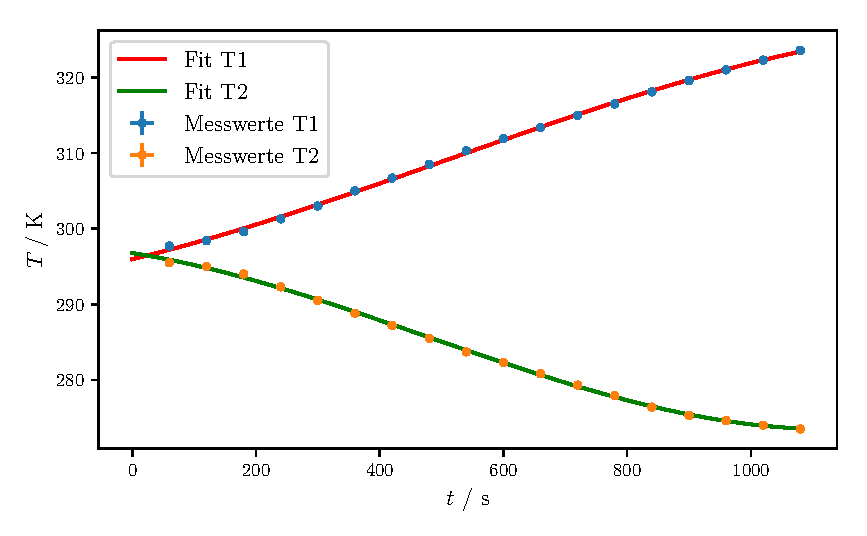
\includegraphics{plot-t-T.pdf}
  \caption{Plot und Fit der Temperaturen in Zeitabhöngigkeit.}
  \label{fig:plot_zeit-temp}
\end{figure}

Die Messwerte in \autoref{tab:zeit-temp} wurden in einem Diagramm dargestellt und mithilfe von Python 3.7.0 durch einen Fit der Form $T(t) = at² + bt + c$ angenähert.
Dieses ist in \autoref{fig:plot_zeit-temp} zu sehen.
%Werte einfügen
Der Differentialquotient $\frac{\text{d}T_1}{\text{d}t}$ beziehungsweise $\frac{\text{d}T_2}{\text{d}t}$ lässt sich als
\\ \\
\centerline{$T'_1 = 2at + b$}
\\ \\
bestimmen. 
Der Fehler dieser Größen lässt sich mithilfe der Gauß'schen Fehlerfortpflanzung
\begin{equation}
  \label{eqn:fehlerfortpflanzung}
  \sigma_\text{u}^2 = \sum\!\bigg(\frac{\partial u}{\partial x_i}\bigg)^2 \! \sigma_i^2
\end{equation}
berechnen.
In diese werden die Werte eingesetzt, um so $\sigma_\text{$T'_1$}$ und $\sigma_\text{$T'_2$}$ zu berechnen:
\\ \\ %Fehlerrechnung einfügen
\centerline{$\sigma_\text{$T'_1$} = \sqrt{a}$}
\\ \\
Somit finden sich die Werte, die in \autoref{tab:temp-temp-ableitung} zu sehen sind. 
%zeiten 180 540 720 1020
\begin{table}[!htp]
  \centering
  \caption{Die errechnten Änderungen der Temperaturen.}
  \label{tab:temp-temp-ableitung}
  \begin{tabular}{
    S[table-format=3.1] @{${}\pm{}$} S[table-format=1.1]
    S[table-format=3.1] @{${}\pm{}$} S[table-format=1.1]
    S[table-format=1.4] @{${}\pm{}$} S[table-format=1.0]
    S[table-format=2.4] @{${}\pm{}$} S[table-format=1.0]}
    \toprule
    \multicolumn{2}{c}{$T_1$ / K} & \multicolumn{2}{c}{$T_2$ / K} & \multicolumn{2}{c}{$T'_1$ / K} & \multicolumn{2}{c}{$T'_2$ / K} \\
    \midrule
    301.3 & 0.1 & 292.3 & 0.1 & 0.0280 & 0 & -0.0280 & 0 \\
    310.3 & 0.1 & 283.7 & 0.1 & 0.0268 & 0 & -0.0242 & 0 \\
    315.0 & 0.1 & 279.3 & 0.1 & 0.0258 & 0 & -0.0212 & 0 \\
    322.3 & 0.1 & 274.0 & 0.1 & 0.0248 & 0 & -0.0181 & 0 \\
    \bottomrule
  \end{tabular}
\end{table}

Des weiteren lässt sich die Wärmekapazität des Wassers $C_w$ mit
\\ \\
\centerline{$C_w = m_w c_w = \rho_w V_w c_w$}
\\ \\
berechnen. Dabei ist $c_w = 4.182 \frac{\textrm{kJ}}{\textrm{kg$\cdot$K}}$ in der Literatur zu finden. ZITAT
Der Fehler wird mithilfe von \eqref{eqn:fehlerfortpflanzung} errechnet:
\\ \\
\centerline{$\sigma_\text{$C_w$} = \rho_w c_w \sigma_V$}
\centerline{$C_w = (12.5 \pm 0.5) \cdot 10³ \frac{\textrm{J}}{\textrm{K}}$}
\\ \\
Die Wärmekapazität der Kupferschlange und des Behälters $C_k$ beträgt 
\\ \\
\centerline{$C_k = m_k c_k = 750 \frac{\textrm{J}}{\textrm{K}}$.}
\\ \\
Diese Werte werden in GLEICHUNG eingsetzt, um so die Güteziffern $\nu$ zu errechnen. 
Dieser Fehler $\sigma_\nu$ dieses lässt sich ebenfalls mithilfe von Gleichung \eqref{eqn:fehlerfortpflanzung} berechnen.
\\ \\
\centerline{$\sigma_\nu^2 = 1 \cdot \sigma_\text{$T'_1$}^2 + \bigg(\frac{\text{d}T_1}{\text{d}t}\bigg)^2 \sigma_\text{$C_w$}^2$}
\\ \\
Diese sind in \autoref{tab:temp-guete} zu finden.

\begin{table}[!htp]
  \centering
  \caption{Die Güteziffern bei unterschiedlichen Temperaturen.}
  \label{tab:temp-guete}
  \begin{tabular}{
    S[table-format=3.1] @{${}\pm{}$} S[table-format=1.0]
    S[table-format=1.3] @{${}\pm{}$} S[table-format=1.0]
    S[table-format=2.3]}
    \toprule
    \multicolumn{2}{c}{$T_1$ / K} & \multicolumn{2}{c}{$\nu$} & {$\nu_\text{ideal}$} \\
    \midrule
    301.3 & 0.1 & 1.903 & 0 & 41.274 \\
    310.3 & 0.1 & 1.732 & 0 & 11.665 \\
    315.0 & 0.1 & 1.627 & 0 &  8.824 \\
    322.3 & 0.1 & 1.528 & 0 &  6.673 \\
    \bottomrule
  \end{tabular}
\end{table}

\begin{table}[!htp]
    \centering
    \caption{Temperatur und Druck im Verhältnis.}
    \label{tab:temp-druck}
    \begin{subtable}{0.48\textwidth}
        \begin{tabular}{
            S[table-format=3.1] @{${}\pm{}$} S[table-format=2.1]
            S[table-format=1.1] @{${}\pm{}$} S[table-format=1.1]}
            \toprule
            \multicolumn{2}{c}{$T_1$ / K} & \multicolumn{2}{c}{$p_a$ / $10^5$pa} \\
            \midrule
            297.7 & 0.1 &  7.5 & 0.5 \\
            298.4 & 0.1 &  7.8 & 0.5 \\
            299.6 & 0.1 &  8.0 & 0.5 \\
            301.3 & 0.1 &  8.5 & 0.5 \\
            303.0 & 0.1 &  8.8 & 0.5 \\
            305.0 & 0.1 &  9.2 & 0.5 \\
            306.7 & 0.1 &  9.5 & 0.5 \\
            308.5 & 0.1 & 10.0 & 0.5 \\
            310.3 & 0.1 & 10.1 & 0.5 \\
            311.9 & 0.1 & 10.5 & 0.5 \\
            313.4 & 0.1 & 10.9 & 0.5 \\
            315.0 & 0.1 & 11.2 & 0.5 \\
            316.5 & 0.1 & 11.5 & 0.5 \\
            318.1 & 0.1 & 12.0 & 0.5 \\
            319.6 & 0.1 & 12.5 & 0.5 \\
            321.0 & 0.1 & 12.8 & 0.5 \\
            322.3 & 0.1 & 13.1 & 0.5 \\
            323.6 & 0.1 & 13.5 & 0.5 \\
            \bottomrule
        \end{tabular}
        \caption{Reservoir 1}
    \end{subtable}
    \begin{subtable}{0.48\textwidth}
        \centering
        \begin{tabular}{S[table-format=3.1] c S[table-format=1.1] S[table-format=1.1] c S[table-format=1.1]}
            \toprule
            \multicolumn{2}{c}{$T_2$ / K} & \multicolumn{2}{c}{$p_b$ / $10^5$pa} \\
            \midrule
            295.5 & 0.1 & 2.8 & 0.2 \\
            295.0 & 0.1 & 2.9 & 0.2 \\
            294.0 & 0.1 & 3.0 & 0.2 \\
            292.3 & 0.1 & 3.2 & 0.2 \\
            290.5 & 0.1 & 3.2 & 0.2 \\
            288.8 & 0.1 & 3.2 & 0.2 \\
            287.2 & 0.1 & 3.2 & 0.2 \\
            285.5 & 0.1 & 3.2 & 0.2 \\
            283.7 & 0.1 & 3.2 & 0.2 \\
            282.3 & 0.1 & 3.2 & 0.2 \\
            280.8 & 0.1 & 3.2 & 0.2 \\
            279.3 & 0.1 & 3.2 & 0.2 \\
            277.9 & 0.1 & 3.2 & 0.2 \\
            276.4 & 0.1 & 3.2 & 0.2 \\
            275.3 & 0.1 & 3.3 & 0.2 \\
            274.6 & 0.1 & 3.3 & 0.2 \\
            274.0 & 0.1 & 3.3 & 0.2 \\
            273.5 & 0.1 & 3.3 & 0.2 \\
            \bottomrule
        \end{tabular}
        \caption{Reservoir 2}
    \end{subtable}
\end{table}

\begin{figure}
  \centering
  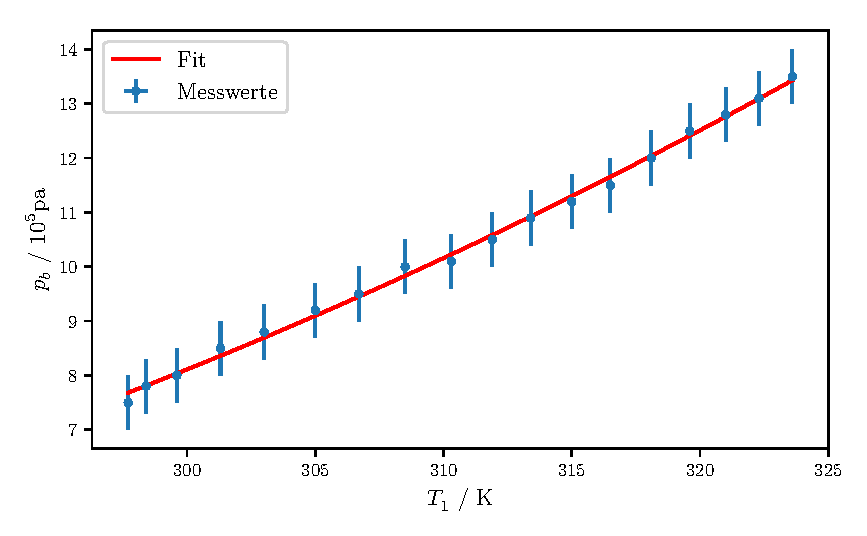
\includegraphics{plot-T-p1.pdf}
  \caption{Die Temperaturen und der Druck in Reservoir 1 gegeneinander aufgetragen.}
  \label{fig:plot_temp-druck1}
\end{figure}

\begin{figure}
  \centering
  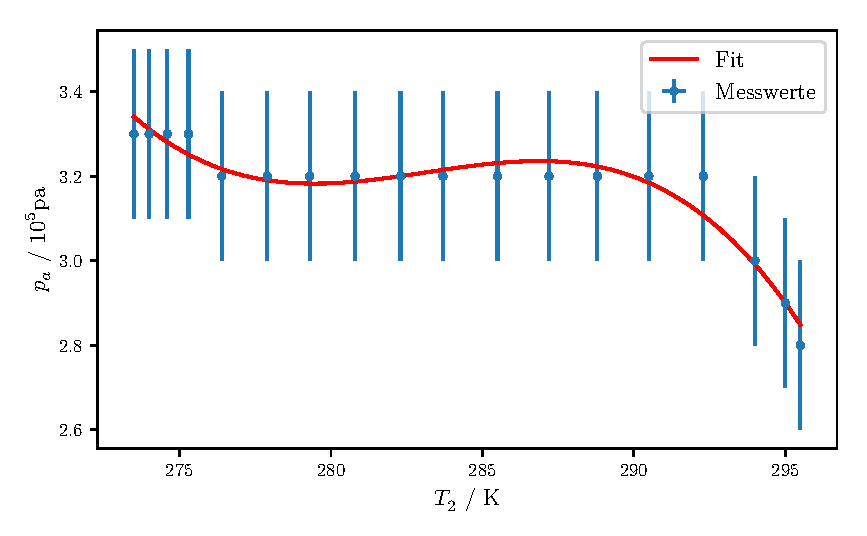
\includegraphics{plot-T-p2.pdf}
  \caption{Die Temperaturen und der Druck in Reservoir 2 gegeneinander aufgetragen.}
  \label{fig:plot_temp-druck2}
\end{figure}

Zur Bestimmung des Massendurchsatzes muss zuvor die Verdampfungswärme L des Gases bestimmt werden. Dies geschieht, in dem zuvor vom Manometer aufgenommene
Druck-Temperetur Wertepaare gegeneinander aufgetragen werden und hierüber eine lineare Ausgleichsrechnung erfolgt. Die Wertepaare hierzu finden sich in \autoref {tab:temppa}.
Die Verdampfungswärme L lässt sich dann durch die Steigung $a$ der linearen Ausgleichsgeraden und der Gaskonstanten $R$ durch $L = m \cdot R$, wobei die Ausgleichsgerade durch
\begin{equation}
  \label{eqt:Ausgleichsgerade}
  y = a \cdot x + b,
\end{equation}
wobei y hier der Druck und x die Temperatur, womit a die Zunahme des Druckes bei steigender Temperatur und b den Druck bei $ T = 0$.
Die Parameter ergeben sich durch
\begin{equation}
\label{eqt:b}
  b = \frac {\sum_{i=1}^n (x_i - \overline{x}) \cdot (y_i - \overline{y})}{\sum_{i=1}^n (x_i - \overline{x})^2}
\end{equation}
und 
\begin{equation}
\label{eqt:a}
  a = \overline{y} - b \cdot \overline{x}, 
\end{equation}
wobei $x_i$ die Temperaturwerte und $y_i$ die Druckwerte (beides zu sehen in \autoref{tab:temppa}) sind. Die dazugehörigen Mittelwerte $\overline{x}$ und $\overline{y}$, zu n Werten (hier: $n = 10$), berechnen sich über
\begin{equation}
\label{eqt:mittelwert}
  \overline{x} = \frac {1}{n} \sum_{i=1}^n x_i . 
\end{equation}
Somit ergeben sich nach Gleichungen \eqref{eqt:b}, \eqref{eqt:a} und \eqref{eqt:mittelwert}
\begin{equation}
    b = 17570,99
\end{equation}
und 
\begin{equation}
 \lvert a \rvert = 4552563,3 . 
\end{equation}
Die sich dadurch nach Gleichung \eqref{eqt:Ausgleichsgerade} ergebene Gerade ist in Abbildung \ref{fig:dampf} zu sehen.
Zur Bestimmung von L ist neben der Steigung der Verdampfungkurve, die Gaskonstante $R = 8,314 \frac{\symup{J}}{\symup{mol} \symup{K}}$ nötig.
Mit der Relation
\begin{equation}
  L = \lvert a \rvert R
\end{equation}
lässt sich die Verdampfungswärme als
\begin{equation}
  L = 37850011,28 \frac{\symup{J}}{\symup{mol} \symup{K}}
\end{equation}
berechnen.
Zur weiteren Berechnung muss die Verdampfungswärme durch die molare Masse geteilt werden, um L in einer zur weiteren Berechnung sinnvollen Einheit zu erhalten, wobei 
die molare Masse von Dichlordiflourmethan $M = 120,91 \frac{\symup{g}}{\symup{mol} }$ \cite{chemie} beträgt, womit
\begin{equation}
  L =  313042,85236953106 \frac{\symup{J}}{\symup{g} \symup{K}}
\end{equation}
beträgt. Nach \eqref{eqt:massendurchsatz} berechnen sich dann die Massendurchsätze, wie in \autoref{unknown} zusehen.

\begin{table}[!htp]
\centering
\caption{Die Temperatur - Druck Wertepaare.}
\label{tab:temppa}
\begin{tabular}{c c}
\toprule $p$ / bar & $T$ / K \\
\midrule
3.0 & 273.15 \\
3.8 & 279.15 \\
4.0 & 281.15 \\
4.8 & 287.15 \\
5.5 & 293.15 \\
6.0 & 295.15 \\
7.0 & 301.15 \\
7.4 & 303.15 \\
9.5 & 313.15 \\
12.0& 323.15 \\
\bottomrule
\end{tabular}
\end{table}

\begin{figure}
  \centering
  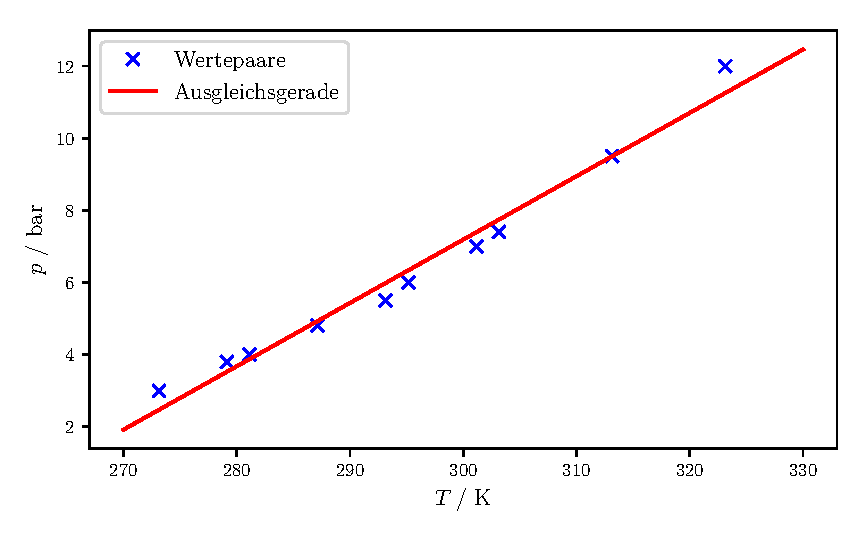
\includegraphics{plot-L.pdf}
  \caption{Verdampfungkurve zu L.}
  \label{fig:dampf}
\end{figure}
\begin{table}[!htp]
\centering
\caption{Die vom Kompressor genutzte elektrische Leistung.}
\label{tab:zeit-leistung}
\begin{tabular}{S[table-format=4.0] @{${}\pm{}$} S[table-format=1.0] S[table-format=3.0] @{${}\pm{}$} S[table-format=1.0]}
\toprule
\multicolumn{2}{c}{$t$ / s} & \multicolumn{2}{c}{$P$ / W} \\
\midrule
  60 & 5 & 175 & 5 \\
 120 & 5 & 180 & 5 \\
 180 & 5 & 190 & 5 \\
 240 & 5 & 195 & 5 \\
 300 & 5 & 200 & 5 \\
 360 & 5 & 200 & 5 \\
 420 & 5 & 205 & 5 \\
 480 & 5 & 205 & 5 \\
 540 & 5 & 205 & 5 \\
 600 & 5 & 205 & 5 \\
 660 & 5 & 205 & 5 \\
 720 & 5 & 210 & 5 \\
 780 & 5 & 210 & 5 \\
 840 & 5 & 215 & 5 \\
 900 & 5 & 215 & 5 \\
 960 & 5 & 215 & 5 \\
1020 & 5 & 215 & 5 \\
1080 & 5 & 215 & 5 \\
\bottomrule
\end{tabular}
\end{table}

\begin{figure}
  \centering
  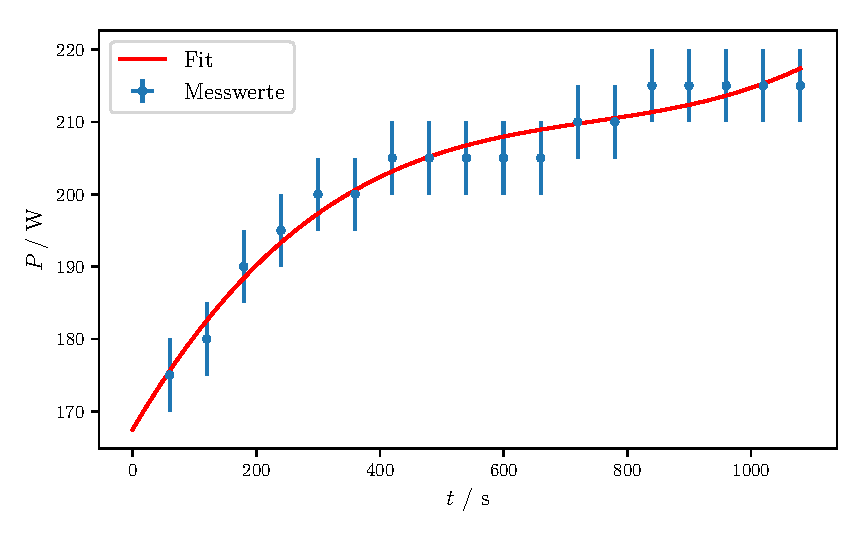
\includegraphics{plot-t-P.pdf}
  \caption{Die elektrische Leistung am Kompressor zu den jeweiligen Zeitpunkten.}
  \label{fig:plot_zeit-druck}
\end{figure}

Die nötigen Werte für die Dichte des Gases $\text{Cl}_\text{2}\text{F}_\text{2}\text{C}$ $\rho_0$ bei 0°C und 1 Bar Druck sowie $\kappa$ lassen sich in der Literatur finden \cite{206}.
\\ \\
\centerline{$\rho_0 = 5.51 \frac{\textrm{kg}}{\textrm{m}^3}$}
\centerline{$\kappa = 1.14$}
\\ \\
Damit und den Werten in \autoref{tab:temp-druck} und \autoref{tab:zeit-leistung} sowie GLEICHUNG ergeben sich die Daten für die mechanische Kompressorleistung in \autoref{tab:mech-kompleistung}.

\begin{table}
  \centering
  \caption{Mechanische Kompressorleistung.}
  \label{tab:mech-kompleistung}
  \begin{tabular}{
    S[table-format=3.1] @{${}\pm{}$} S[table-format=1.0]
    S[table-format=1.0] @{${}\pm{}$} S[table-format=1.0]}
    \toprule
    \multicolumn{2}{c}{$T_1$ / K} & \multicolumn{2}{c}{$P_\text{mech}$} \\
    \midrule
    301.3 & 0.1 & 0 & 0 \\
    310.3 & 0.1 & 0 & 0 \\
    315.0 & 0.1 & 0 & 0 \\
    322.3 & 0.1 & 0 & 0 \\
    \bottomrule
  \end{tabular}
\end{table}